%% m4l motivation

\section{Motivation for the \mFourL{} measurement}
\label{sec:fourlepmotivation}

The four lepton final state is a particularly interesting channel to study as it receives contributions from many physics processes. First and foremost, there is the production of a pair of $Z$-bosons via quark-antiquark interactions in \info[]{s-channel not in SM because it includes neutral $ZZZ$ or $ZZ$\photon vertex} both the $t$- and $u$-channel. The $t$-channel diagram is shown in Figure \ref{fig:m4lfeynman:qqZZ}, and represents, by far, \improvement[]{Read more about why the u-channel diagram is not preferred} the largest contribution to the $ZZ$ production and thus to the \mFourL{} distribution. At the low mass end where $\mFourL{}=m_{Z}$, there is resonant production of a single $Z$ boson via the $s$-channel diagram in Figure \ref{fig:m4lfeynman:singleZ}. At $\mFourL{}=\unit{180}{\GeV}$ and beyond, the threshold for the on-shell production of two $Z$ bosons is reached and results in a peak in the four lepton invariant mass spectrum. 

Second in magnitude is the gluon-induced production of a $Z$ boson pair. This occurs via a triangle or box quark loop, which results in a factor $\alpha_s^2$ suppression. It still plays a substantial role, however, because at small $x$\footnote{Here $x$ is the component of the proton's momentum carried by the struck quark. At the \LHC the protons have very high energies; therefore the \LHC can be described as a small $x$ collider \cite{zotov2012small}} gluon-gluon luminosity is higher than the quark-antiquark luminosity \cite{Glover:194539}. The contribution from this process in on the order of ten percent \cite{Becker:2230817}. Finally in the pool of $Z$ boson pairs there is a small contribution from decaying Higgs bosons, which themselves are produced also via gluon fusion, as illustrated in Figure \ref{fig:m4lfeynman:ggHZZ}. There is resonant Higgs production at \mFourL=\unit{125}{\GeV}, and a non-resonant enhancement at $\mFourL{}=m_{t}=\unit{350}{\GeV}$ from the top quark loop. Beyond \unit{350}{\GeV}, the Higgs-mediated $Z$ boson pair production process destructively interferes with continuum production of on-shell $Z$ bosons \cite{Campbell_2016}.

The \mFourL{} distribution can be a useful probe for certain new physics scenarios. Take for example, the high mass tail of the invariant mass spectrum. This region is dependent on the couplings of the Higgs to incoming and outgoing particles while independent of the Higgs boson width \cite{Campbell_2016}, a unique property that can be exploited to derive model-independent limits on the Higgs couplings, and on the \todo{reword, this is copy pasted} contribution of new states in the Higgs to gluon coupling \cite{Cacciapaglia_2014}. It has also been previously exploited to derive model-independent constraints on the Higgs boson width \cite{Caola_2013}. 
%% Secondly, under specific assumptions a class of models exists for which the off-shell coupling measurement together with a measurement of the on-shell signal strength can be re-interpreted in terms of a bound on the total Higgs boson width. In this paper, we provide a first step towards a classification of the models for which a total width measurement is viable and we discuss examples of BSM models for which the off-shell coupling measurement can be important in either constraining or even discovering new physics in the upcoming LHC runs

A previous iteration of the \mFourL{} by the \ATLAS collaboration using \unit{36}{\invfb} of data can be found in Reference~\cite{Aaboud:2019lxo}. For the analysis presented int his chapter, the data used corresponds to \unit{139}{\invfb} at $\sqrt{2}=13$~TeV, collected by the ATLAS detector during Run 2 of the LHC between 2015 and 2018. Compared to the previous round, the new \mFourL{} measurement takes advantaged of the increased data statistics and focuses on improving inclusivity and acceptance (particularly in the low mass region), and maximizing reinterpretability. Unlike dedicated $ZZ\rightarrow 4\ell$ analyses~\cite{Sirunyan:s10052-018-5567-9,Aaboud:97.032005}, the inclusive \mFourL{} does not have an upper mass cut on the lepton pairs. Both pairs are allowed to be above the $Z$ mass threshold. This chapter presents the measurement in full, with a stronger focus on the unfolding studies on which the author contributed. The analysis is published in Reference~\cite{m4l2021_paper}, from which certain sections are adapted.

\begin{figure}
    \centering
    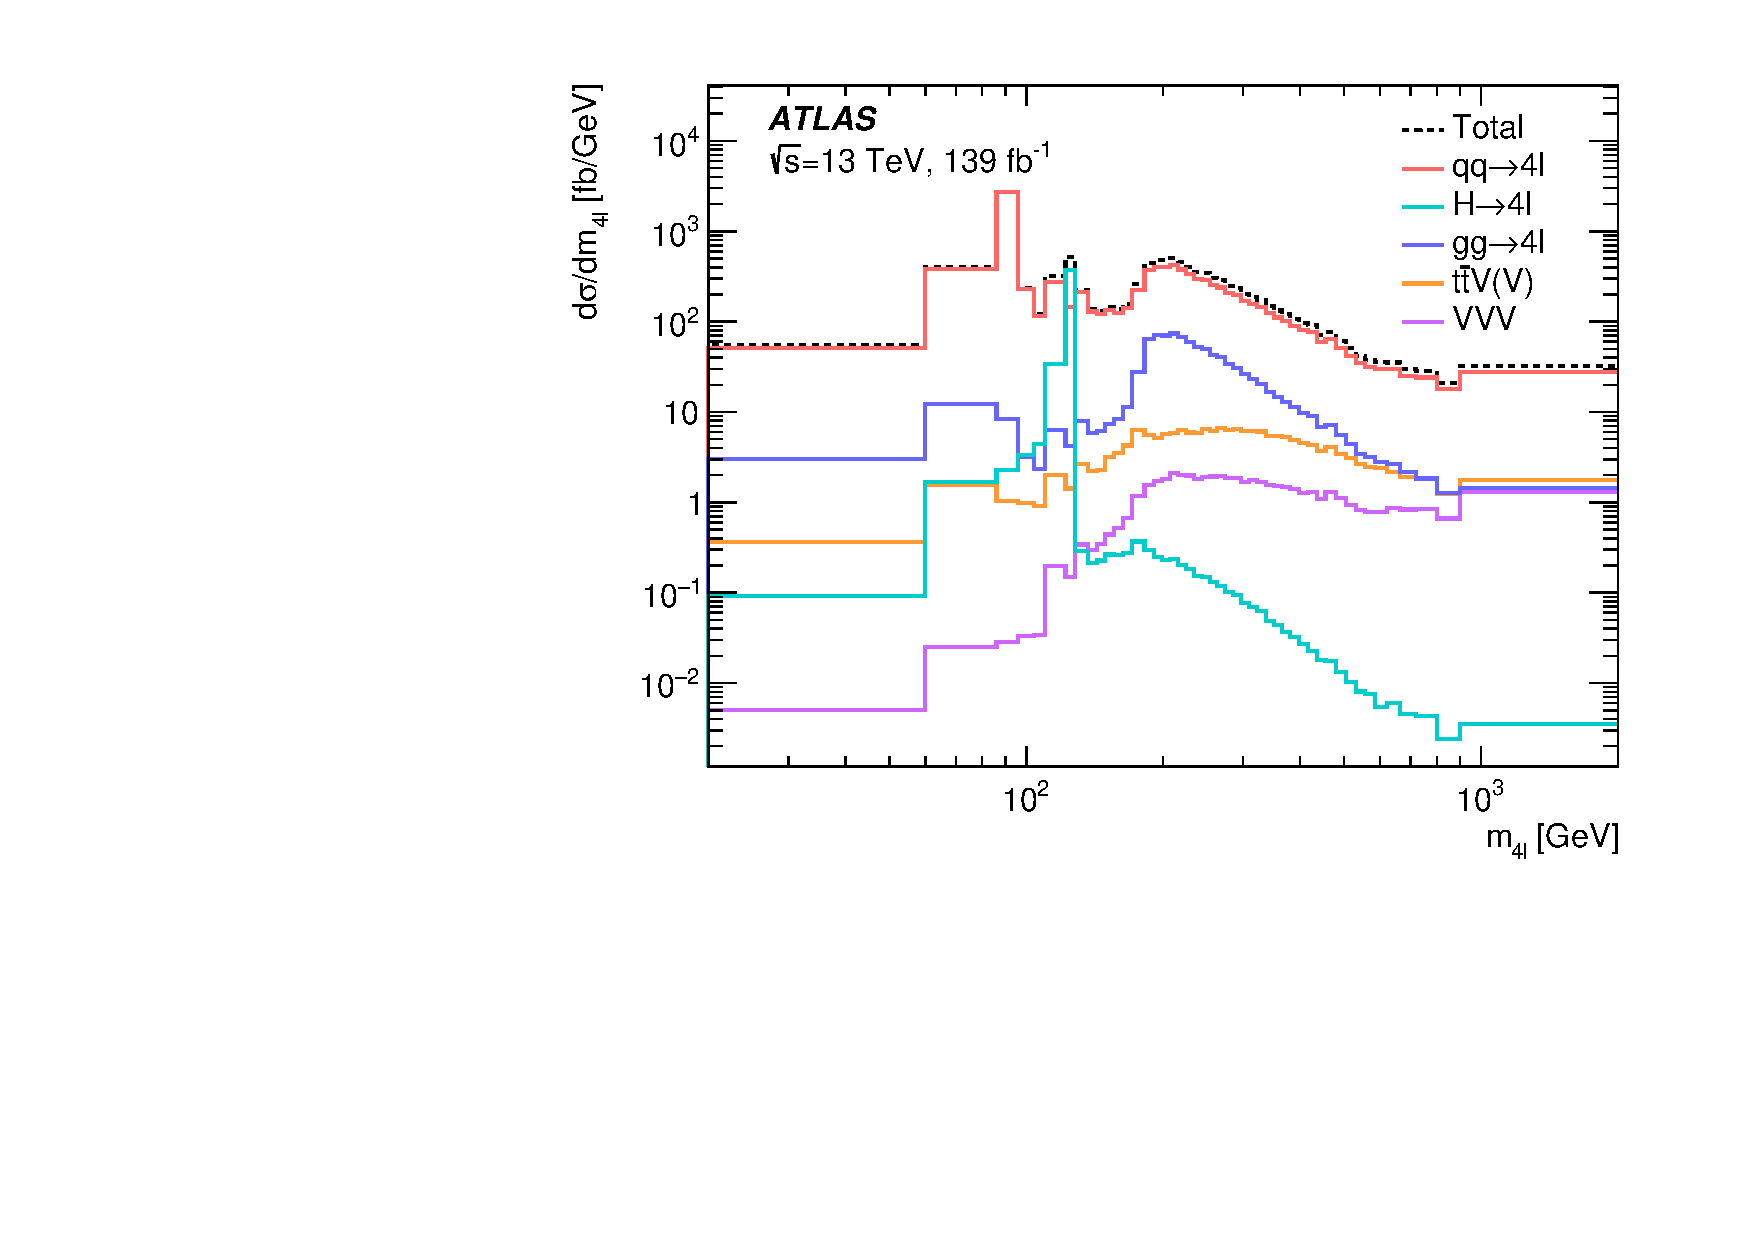
\includegraphics[width=0.7\textwidth]{Figures/m4l/processbreakdown.pdf}
    \caption{Breakdown of contributing processes contributing to the \mFourL{} distribution.}
    \label{fig:m4lbreakdown}
\end{figure}

\begin{figure}
\centering
\begin{subfigure}{.24\textwidth}
  \centering
  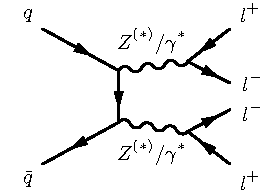
\includegraphics[width=.99\textwidth]{Figures/FeynGraphs/qqZZ4l.pdf}
  \caption{\qqZZ}
  \label{fig:m4lfeynman:qqZZ}
\end{subfigure}%
\begin{subfigure}{.24\textwidth}
  \centering
  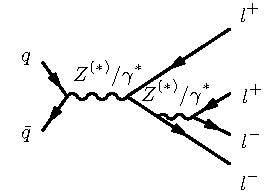
\includegraphics[width=.99\textwidth]{Figures/FeynGraphs/qqZZ4lrad.pdf}
  \caption{A subfigure}
  \label{fig:m4lfeynman:singleZ}
\end{subfigure}
\begin{subfigure}{.24\textwidth}
  \centering
  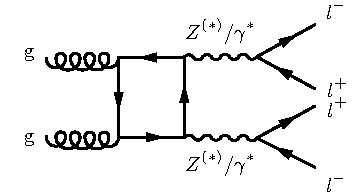
\includegraphics[width=.99\textwidth]{Figures/FeynGraphs/ggZZ4lbox.pdf}
  \caption{A subfigure}
  \label{fig:m4lfeynman:ggZZ}
\end{subfigure}
\begin{subfigure}{.24\textwidth}
  \centering
  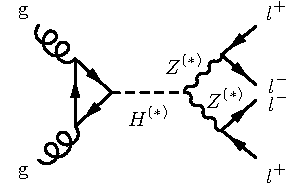
\includegraphics[width=.99\textwidth]{Figures/FeynGraphs/ggZZ4lhiggs.pdf}
  \caption{A subfigure}
  \label{fig:m4lfeynman:ggHZZ}
\end{subfigure}
\caption{Feynman diagrams for quark- and gluon-induced $ZZ$ production. The processes shown are the main contributors. This figure is from Ref.~\cite{m4l2021_paper}.}
\label{fig:m4lfeynman}
\end{figure}

% this channel provides a clean leptonic final state resulting in a small instrumental background, where one or more of the reconstructed lepton candidates originate from the misidentification of jet fragments or from nonprompt leptons.
